% Source: Lecture14.pdf, pages 1-9. The source is titled "Renormalization group in critical
% phenomena" and has no lecture number on the page.
\lecture{14}

A major and far-reaching advance in the understanding of critical phenomena occurred with the
development and application of the renormalization group (RG) in the late 1960s and early 1970s.
(Interestingly, it was also during this time that the RG transformed particle physics and quantum
field theory.) In stat.\ mech., the RG was pioneered by several researchers, including Kadanoff,
Wilson, and Fisher. We will focus much of our discussion on the real-space RG; via a Fourier
transform from position space $\mathbf{x}$ to momentum space $\mathbf{k}$, this has an obvious
analogue in momentum space.

\subsection{The Kadanoff block-spin construction}

We begin with the Kadanoff ``block-spin'' construction. Consider a system undergoing a continuous
phase transition with a correlation length $\xi$ that diverges as $T\to T_c$. The discussion applies
equally well to liquid--gas and magnetic systems, but for definiteness we will focus on magnetic
systems. As $T\to T_c$ and $\xi\to\infty$, there are large domains over which the spins are
correlated. Consider, say, an Ising model on a square or simple cubic lattice, with lattice spacing
$a$. Since the spins are strongly correlated on a length scale $\xi$, one can carry out a block spin
construction as follows. Define $L\times L\equiv b\times b$ blocks. Illustrate for the case
$L\equiv b = 2$.

\begin{diagram}
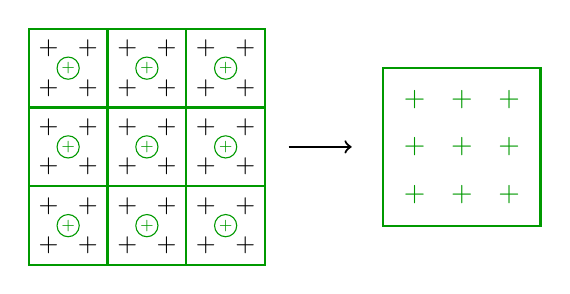
\begin{tikzpicture}[scale=0.5]
  \draw[green!60!black,thick] (0,0) rectangle (6,6);
  \foreach \x in {2,4} \draw[green!60!black,thick] (\x,0) -- (\x,6);
  \foreach \y in {2,4} \draw[green!60!black,thick] (0,\y) -- (6,\y);
  \foreach \x in {0.5,1.5,2.5,3.5,4.5,5.5} \foreach \y in {0.5,1.5,2.5,3.5,4.5,5.5} \node[font=\small] at (\x,\y) {$+$};
  \foreach \x in {1,3,5} \foreach \y in {1,3,5} \node[green!60!black,draw,circle,inner sep=0.5pt,font=\tiny] at (\x,\y) {$+$};
  \draw[->,thick] (6.6,3) -- (8.2,3);
  \begin{scope}[xshift=9cm,yshift=1cm]
    \draw[green!60!black,thick] (0,0) rectangle (4,4);
    \foreach \x in {0.8,2,3.2} \foreach \y in {0.8,2,3.2} \node[green!60!black] at (\x,\y) {$+$};
  \end{scope}
\end{tikzpicture}
\diagramcaption{A $6\times 6$ section of the square lattice $\Lambda_{sq}$ at $T\simeq T_c$, so $\xi\gg a$,
blocked with $L = b = 2$ (left), and the ``blocked'' lattice $\tilde\Lambda_{sq}$ with block spins
$\tilde S_i$ (right). Thus, 4 sites on $\Lambda_{sq}$ are mapped to a single site on the blocked
lattice $\tilde\Lambda_{sq}$.}
\end{diagram}

Procedure: replace each set of 4 spins by a ``block'' spin representing the sum of these 4 spins, with
rescaling, so
\begin{equation}
  \tilde S_i = \sum_{\text{block in }\Lambda_{sq}}s_i .
\end{equation}
A distance $r$ in $\Lambda_{sq}$ is mapped (``renormalized'') to a distance $\tilde r = \frac rL = \frac r2$
on the lattice $\tilde\Lambda_{sq}$.

This blocking or ``decimation'' step can be repeated iteratively. A generalization is to allow a
blocking by a factor $L>2$. This retains the spin information as long as $La\ll\xi$. For a
$d$-dimensional lattice $\Lambda$, $\tilde S_i = L^ds_i$, where $\tilde S_i$ is on the blocked lattice
($\tilde S_i = L^2s_i$ for the 2-dimensional case illustrated above).

At each blocking step, one rewrites the Hamiltonian on the blocked lattice in terms of the $\Ham$ on the
previous lattice. The correlation length $\xi\to\frac\xi L\equiv\frac\xi b$ under a blocking; the
iterative procedure
\begin{equation}
  \Lambda_1\to\underbrace{R(\Lambda_1)}_{\Lambda_2}\to\underbrace{R(R(\Lambda_1))}_{\equiv\Lambda_3}\to\cdots
  \qquad\text{means}\qquad \xi\to\frac\xi b\to\frac{\xi}{b^2}\to\cdots,
\end{equation}
so the $\infty$ iteration of the RG blocking transformation has a fixed point (RGFP) if $\xi = \infty$,
which is the critical point. (Formally, there is also a critical point with $\xi = 0$, namely at
$T = \infty$.)

\subsection{Scaling hypothesis and the thermal and magnetic exponents}

Kadanoff assumed that the (Gibbs) free energy can be rewritten in the same form, with different
parameters in $\Ham$, and with a $(d,L)$-dependent volume factor $L^d$, since here we deal with the total
free energy. Let $\tau = (T-T_c)/T_c$. Then this means
\begin{equation}
  G(\tilde\tau,\tilde H) = L^dG(\tau,H),
\end{equation}
where
\begin{equation}
  \tilde\tau = \varphi_\tau(L)\,\tau,\qquad \tilde H = \varphi_h(L)\,H,
  \qquad\text{such that}\quad \varphi_\tau(1) = 1,\quad \varphi_h(1) = 1 .
\end{equation}
As $T\to T_c$, $\xi\to\infty$, so the original and the blocked systems should go critical together, so
we expect $\tilde\tau\propto\tau$ and $\tilde H\propto H$; this property is incorporated in the above
relations connecting $\tau$ and $\tilde\tau$, and $H$ and $\tilde H$. Further, Kadanoff hypothesized
that
\begin{equation}
  \varphi_\tau(L) = L^{y_\tau}\qquad\text{and}\qquad \varphi_h(L) = L^{y_h}
\end{equation}
($y_\tau$ is often written as $y_t$ or $y_\epsilon$). This ansatz defines the thermal exponent $y_\tau$
and the magnetic exponent $y_h$. From this ansatz and the associated real-space RG, one can derive
important relations between critical exponents. Fundamentally, one sees that, just as one must tune 2
parameters to get critical behavior at a (bi)critical point ($H = H_c = 0$ and $T = T_c$ for magnetic
systems, or $p = p_c$, $T = T_c$ for liquid--gas systems), so also, the critical singularities only
depend on 2 basic exponents. So $\alpha = \alpha'$, $\beta$, $\gamma = \gamma'$, $\nu = \nu'$, $\delta$,
and $\eta$ are all functions of just $y_\tau$ and $y_h$.

Next, Kadanoff hypothesized that the (Gibbs) free energy is a ``generalized homogeneous function'':
with $\tilde\tau = \varphi_\tau(L)\tau = L^{y_\tau}\tau$ and $\tilde H = \varphi_h(L)H = L^{y_h}H$,
\begin{equation}
  G(L^{y_\tau}\tau,L^{y_h}H) = L^dG(\tau,H).
\end{equation}

\subsubsection*{Some mathematical background}

\paragraph{Definition.} $f(x,y)$ is a homogeneous function if $f(\lambda x,\lambda y) = \lambda^pf(x,y)$
for some power $p$. E.g.\ $f(x,y) = x^2+2xy+3y^2$ is a homogeneous function with $p = 2$, since
$f(\lambda x,\lambda y) = (\lambda x)^2+2(\lambda x)(\lambda y)+3(\lambda y)^2 = \lambda^2(x^2+2xy+3y^2) = \lambda^2f(x,y)$.
$f(x,y) = x\sin y$ is not a homogeneous function, since there is no $p$ such that
$f(\lambda x,\lambda y) = \lambda x\cdot\sin(\lambda y) = \lambda^p\cdot x\sin y$.

\paragraph{Definition.} $f(x,y)$ is a generalized homogeneous function if, $\forall\,\lambda\ne 0$,
$\exists\,a\ne 0$ and $b\ne 0$ such that
\begin{equation}
  f(\lambda^ax,\lambda^by) = \lambda f(x,y).
\end{equation}
N.B.: if a function $f(x,y)$ satisfies $f(\mu^{a'}x,\mu^{b'}y) = \mu^{c'}f(x,y)$ then this can be put
into the above form by letting $\mu^{c'} = \lambda$, i.e.\ $\mu = \lambda^{1/c'}$, so
$\mu^{a'} = \lambda^{a'/c'}$, $\mu^{b'} = \lambda^{b'/c'}$, so
$f(\mu^{a'}x,\mu^{b'}y) = f(\lambda^{a'/c'}x,\lambda^{b'/c'}y) = \lambda f(x,y)$, so, with $a'/c' = a$
and $b'/c' = b$, this gives $f(\lambda^ax,\lambda^by) = \lambda f(x,y)$. (If $c' = 0$, then $f$ has a
generalized scale invariance.)

E.g.\ $f(x,y) = x+y^2$ is a generalized homogeneous function with $a = 1$ and $b = \frac12$, since
$f(\lambda^ax,\lambda^by) = f(\lambda x,\sqrt\lambda y) = \lambda x + (\sqrt\lambda y)^2 = \lambda(x+y^2) = \lambda f(x,y)$.
(This definition can be generalized to a function of $n$ variables: $f(x_1,\ldots,x_n)$ is a generalized
homogeneous function if $\exists\,\{a_1,\ldots,a_n\}$ such that
$f(\lambda^{a_1}x_1,\lambda^{a_2}x_2,\ldots,\lambda^{a_n}x_n) = \lambda f(x_1,\ldots,x_n)$, but here we only
need the $n = 2$ case.)

An important property of a generalized homogeneous function $f(x,y)$ is the following. Given that
$f(\lambda^ax,\lambda^by) = \lambda f(x,y)$, let us choose $\lambda = y^{-1/b}$;
\begin{equation}
  \Rightarrow\ f\left(y^{-a/b}x,(y^{-1/b})^by\right) = f\left(\frac{x}{y^{a/b}},1\right) = y^{-1/b}f(x,y),
\end{equation}
so
\begin{equation}
  f(x,y) = y^{1/b}f\left(\frac{x}{y^{a/b}},1\right) = y^{1/b}g\left(\frac{x}{y^{a/b}}\right),
  \qquad\text{where}\quad g\left(\frac{x}{y^{a/b}}\right)\equiv f\left(\frac{x}{y^{a/b}},1\right),
\end{equation}
and $x/y^{a/b}$ is the scaling variable. A generalized homogeneous function of 2 variables can thus be
expressed as a prefactor times a function of 1 variable, $g$. This function $g$ is called the
\emph{scaling function}. We will use this property to derive relations among the critical exponents at a
continuous phase transition (with an $\infty$ correlation length). See, e.g., the book by Stanley,
chapters 11 and 12, for a corresponding discussion.

\subsection{Exponent relations from scaling}

Write the original relation in the canonical form: $G(L^{y_\tau}\tau,L^{y_h}H) = L^dG(\tau,H)$; set
$\lambda = L^d$, so
\begin{equation}
  L^{y_\tau} = (L^d)^{y_\tau/d}\equiv\lambda^{a_\tau},\quad a_\tau = \frac{y_\tau}{d};\qquad
  L^{y_h} = (L^d)^{y_h/d}\equiv\lambda^{a_h},\quad a_h = \frac{y_h}{d};
\end{equation}
then
\begin{equation}\label{eq:Ghom}
  G(\lambda^{a_\tau}\tau,\lambda^{a_h}H) = \lambda G(\tau,H).
\end{equation}
This expresses the Gibbs free energy in canonical form as a generalized homogeneous function.

\paragraph{Magnetization: $\beta$ and $\delta$.} Recall $\dd G(T,H) = -S\dd T - M\dd H$;
$M = -(\partial G/\partial H)_T\equiv-\partial G/\partial H$. Taking $\partial/\partial H$ of the RHS of
eq.~\eqref{eq:Ghom} gives $-\lambda M$. Taking $\partial/\partial H$ of the LHS:
\begin{equation}
  \pder{G(\lambda^{a_\tau}\tau,\lambda^{a_h}H)}{H}
  = \lambda^{a_h}\underbrace{\frac{\partial G(\lambda^{a_\tau}\tau,\lambda^{a_h}H)}{\partial(\lambda^{a_h}H)}}_{-M(\lambda^{a_\tau}\tau,\lambda^{a_h}H)}
  = -\lambda M(\tau,H)
\end{equation}
\begin{equation}\label{eq:Mhom}
  \Rightarrow\quad\boxed{\lambda^{a_h-1}M(\lambda^{a_\tau}\tau,\lambda^{a_h}H) = M(\tau,H)}.
\end{equation}
Now let $H = 0$, $\tau = (T-T_c)/T_c\to 0^-$:
$\Rightarrow\lambda^{a_h-1}M(\lambda^{a_\tau}\tau,0) = M(\tau,0)$; set $\lambda^{a_\tau} = -\frac1\tau$, so
$\lambda = (-\tau)^{-1/a_\tau}$:
\begin{equation}
  \Rightarrow\ \left[(-\tau)^{-1/a_\tau}\right]^{a_h-1}M\left(\left(-\tfrac1\tau\right)\cdot\tau,0\right)
  = (-\tau)^{\frac{1-a_h}{a_\tau}}\underbrace{M(-1,0)}_{\text{const.}} = M(\tau,0).
\end{equation}
Equating this to the form $M(\tau)\propto(-\tau)^\beta$ as $\tau\to 0^-$, we deduce
\begin{equation}
  \boxed{\beta = \frac{1-a_h}{a_\tau}}.
\end{equation}
This expresses the critical exponent $\beta$ in terms of the thermal and magnetic exponents.

Next, in eq.~\eqref{eq:Mhom}, set $\tau = 0$ and $H\to 0$, so, for the critical isotherm (take $H>0$ so
$M>0$),
\begin{equation}
  \lambda^{a_h-1}M(0,\lambda^{a_h}H) = M(0,H) = H^{1/\delta};
\end{equation}
set $\lambda = H^{-1/a_h}$, so
$(H^{-1/a_h})^{a_h-1}\underbrace{M(0,\tfrac HH)}_{M(0,1),\ \text{const.}} = H^{1/\delta}$
$\Rightarrow\frac{1-a_h}{a_h} = \frac1\delta$,
\begin{equation}
  \boxed{\delta = \frac{a_h}{1-a_h}}
  \qquad\Rightarrow\qquad
  \boxed{\beta\delta = \frac{a_h}{a_\tau} = \frac{y_h}{y_\tau}}.
\end{equation}
Solving for $a_h$: $(1-a_h)\delta = a_h$, $\delta = a_h(1+\delta)$ $\Rightarrow$
\begin{equation}
  \boxed{a_h = \frac{\delta}{1+\delta},\qquad a_\tau = \frac{a_h}{\beta\delta} = \frac{1}{\beta(1+\delta)}}.
\end{equation}
So the critical exponent $\delta$ is determined completely in terms of $a_h = y_h/d$; this is
understandable since $T = T_c$, so $\delta$ does not depend on the exponent $y_\tau$ describing the
approach to $T_c$. We continue in this way to determine the other critical exponents in terms of
$a_\tau$ and $a_h$, or equivalently, $y_\tau$ and $y_h$.

\paragraph{Susceptibility: $\gamma$.} From $G(\lambda^{a_\tau}\tau,\lambda^{a_h}H) = \lambda G(\tau,H)$, we
got, by taking $\partial/\partial H$, the equation
$\lambda^{a_h-1}M(\lambda^{a_\tau}\tau,\lambda^{a_h}H) = M(\tau,H)$. Next, take $\partial/\partial H$ again:
the susceptibility is $\chi = \pder{M}{H} = -\frac{\partial^2G}{\partial H^2}$, and
\begin{equation}
  \lambda^{a_h-1}\pder{M(\lambda^{a_\tau}\tau,\lambda^{a_h}H)}{H} = \chi(\tau,H).
\end{equation}
LHS:
\begin{equation}
  \lambda^{2a_h-1}\underbrace{\frac{\partial M(\lambda^{a_\tau}\tau,\lambda^{a_h}H)}{\partial(\lambda^{a_h}H)}}_{\chi(\lambda^{a_\tau}\tau,\lambda^{a_h}H)} = \chi(\tau,H)
  \quad\Rightarrow\quad \lambda^{2a_h-1}\chi(\lambda^{a_\tau}\tau,\lambda^{a_h}H) = \chi(\tau,H).
\end{equation}
Set $\lambda = \tau^{-1/a_\tau}$, so
$\left[\tau^{-1/a_\tau}\right]^{2a_h-1}\chi\left(\left(\frac1\tau\right)\tau,\tau^{-a_h/a_\tau}H\right) = \chi(\tau,H)$;
set $H = 0$ to get the critical behavior as $\tau\to 0$:
\begin{equation}
  \tau^{\frac{1-2a_h}{a_\tau}}\underbrace{\chi(1,0)}_{\text{const.}} = \chi(\tau,0) = \tau^{-\gamma}
  \quad\Rightarrow\quad\boxed{\gamma = \frac{2a_h-1}{a_\tau}},
\end{equation}
similarly with $\boxed{\gamma' = \gamma}$.

Now recall that $\beta = \frac{1-a_h}{a_\tau}$ and $\delta = \frac{a_h}{1-a_h}$, so
$\delta - 1 = \frac{a_h-(1-a_h)}{1-a_h} = \frac{2a_h-1}{1-a_h}$, and hence
\begin{equation}
  \beta(\delta-1) = \left(\frac{1-a_h}{a_\tau}\right)\left(\frac{2a_h-1}{1-a_h}\right) = \frac{2a_h-1}{a_\tau} = \gamma,
\end{equation}
so
\begin{equation}
  \boxed{\beta(\delta-1) = \gamma},\quad\text{i.e.}\quad\boxed{\beta\delta = \beta+\gamma}.
\end{equation}
Check: Landau--Ginzburg or MFT $\Rightarrow\beta = \frac12$, $\delta = 3$, $\gamma = 1$, so
$\beta\delta = \frac32 = \frac12+1$ \checkmark; LG/MFT obeys this exponent relation.
2D Ising ($q = 2$ Potts) $\Rightarrow\beta = \frac18$, $\delta = 15$, $\gamma = \frac74$, so
$\beta\delta = \frac{15}{8}$; $\beta+\gamma = \frac18+\frac74 = \frac{15}{8}$, so the 2D Ising model also
obeys this relation. 2D $q = 3$ Potts $\Rightarrow\beta = \frac19$, $\delta = 14$, $\gamma = \frac{13}{9}$,
so $\beta\delta = \frac{14}{9}$; $\beta+\gamma = \frac{14}{9}$, OK.

\paragraph{Specific heat: $\alpha$.} We can also differentiate with respect to $T$, or equivalently
$\tau$, to get $U$ and $C_H$: $\dd G = -S\dd T - M\dd H$;
$S = -(\partial G/\partial T)_H$,
$C_H = T(\partial S/\partial T)_H = -T(\partial^2G/\partial T^2)_H$. With $\tau = (T-T_c)/T_c$,
$\partial\tau/\partial T = 1/T_c$, $\frac{\partial}{\partial T} = \frac{1}{T_c}\frac{\partial}{\partial\tau}$,
so $C_H = -\frac{T}{T_c^2}\left(\frac{\partial^2G}{\partial\tau^2}\right)_H$. From
$G(\lambda^{a_\tau}\tau,\lambda^{a_h}H) = \lambda G(\tau,H)$, we have
\begin{equation}
  \underbrace{\lambda^{2a_\tau}\left(\frac{T}{T_c^2}\right)\frac{\partial^2G(\lambda^{a_\tau}\tau,\lambda^{a_h}H)}{\partial(\lambda^{a_\tau}\tau)^2}}_{-\lambda^{2a_\tau}C_H(\lambda^{a_\tau}\tau,\lambda^{a_h}H)}
  = \left(\frac{T}{T_c^2}\right)\lambda\frac{\partial^2G(\tau,H)}{\partial\tau^2} = -\lambda C_H(\tau,H),
\end{equation}
so
\begin{equation}
  \lambda^{2a_\tau-1}C_H(\lambda^{a_\tau}\tau,\lambda^{a_h}H) = C_H(\tau,H).
\end{equation}
Set $H = 0$, let $\tau\to 0$, set $\lambda = \tau^{-1/a_\tau}$ $\Rightarrow$
\begin{equation}
  \left[\tau^{\frac{1-2a_\tau}{a_\tau}}\right]C_H\left((\tau^{-1/a_\tau})^{a_\tau}\tau,0\right) = C_H(\tau,0) = \tau^{-\alpha}
  \quad\Rightarrow\quad\boxed{\alpha = 2-a_\tau^{-1} = \frac{2a_\tau-1}{a_\tau}},
\end{equation}
similarly with $\alpha' = \alpha$. The fact that $\alpha = \alpha'$ depends only on $a_\tau$ and not on
$a_h$ follows because $H$ has already been set equal to its value at the critical point, $H = 0$.

Summarizing: $\boxed{\alpha' = \alpha}$. Then
\begin{equation}
  \alpha+2\beta+\gamma = \left(2-\frac{1}{a_\tau}\right) + 2\left(\frac{1-a_h}{a_\tau}\right) + \left(\frac{2a_h-1}{a_\tau}\right) = 2,
\end{equation}
\begin{equation}
  \boxed{\alpha+2\beta+\gamma = 2}\qquad\text{(Rushbrooke relation)}.
\end{equation}
E.g.\ LG/MFT: $\alpha = 0$ (disc.), $\beta = \frac12$, $\gamma = 1$ \checkmark; 2D Ising: $\alpha = 0$
(log div.), $\beta = \frac18$, $\gamma = \frac74$ $\Rightarrow 0+2(\frac18)+\frac74 = 2$ \checkmark.

From the relations expressing $a_h$ in terms of $\delta$ and $a_\tau$ in terms of $\beta$ and $\delta$, one
obtains the fundamental magnetic and thermal exponents:
\begin{equation}
  a_\tau = \frac{1}{\beta(\delta+1)}\ \text{and}\ y_\tau = a_\tau\cdot d;\qquad
  a_h = \frac{\delta}{\delta+1}\ \text{and}\ y_h = a_h\cdot d .
\end{equation}
E.g.\ LG/MFT $\Rightarrow\beta = \frac12$, $\delta = 3$ $\Rightarrow a_\tau = \frac{1}{\frac12\cdot 4} = \frac12$,
$a_h = \frac34$. 2D Ising ($q = 2$ Potts): $\beta = \frac18$, $\delta = 15$ $\Rightarrow
a_\tau = \frac{1}{\frac18\cdot 16} = \frac12$, $a_h = \frac{15}{16}$, $y_h = a_h\cdot d = \frac{15}{8}$,
$y_\tau = a_\tau\cdot d = 1$.

\paragraph{Correlation length: $\nu$ (hyperscaling).} Recall that the correlation length diverges as
\begin{equation}
  \xi\sim\begin{cases}\tau^{-\nu} & T>T_c\\ (-\tau)^{-\nu'} & T<T_c .\end{cases}
\end{equation}
Now the second derivative of the free energy with respect to $T$ or $\tau$ gives the specific heat
capacity $C_H$, which has the singular behavior
$C_H\sim\begin{cases}\tau^{-\alpha} & T>T_c\\ (-\tau)^{-\alpha'} & T<T_c\end{cases}$ as $\tau\to 0$. This
means that $G(T,0)$ must have a finite non-analyticity at $\tau = 0$. Consistent with the Kadanoff
construction, one can write $G(\tau,H=0)_{\text{sing.}}\sim(L/\xi)^d$; now since $\xi\sim\tau^{-\nu}$ for
$\tau>0$, this is
\begin{equation}
  G(\tau,H=0)_{\text{sing.}}\sim\xi^{-d}\sim(\tau^{-\nu})^{-d}\sim\tau^{d\nu}\sim\tau^{2-\alpha},
\end{equation}
since two derivatives with respect to $\tau$ $\Rightarrow C_H\sim\tau^{-\alpha}$
\begin{equation}
  \Rightarrow\quad\boxed{d\nu = 2-\alpha};\qquad\text{similarly,}\quad\boxed{d\nu' = 2-\alpha'}.
\end{equation}
Combining this with $\alpha = \alpha' = 2-a_\tau^{-1}$ $\Rightarrow d\nu = 2-(2-a_\tau^{-1})\Rightarrow
d\nu = \frac{1}{a_\tau} = \frac{d}{y_\tau}\Rightarrow\nu = \frac{1}{y_\tau}$, and similarly
$d\nu' = \frac{d}{y_\tau}$ $\Rightarrow$
\begin{equation}
  \boxed{\nu' = \nu = \frac{1}{y_\tau}}.
\end{equation}

\paragraph{Correlation function: $\eta$.} A corresponding analysis of the critical behavior of the 2-spin
correlation function yields the exponent relations
\begin{equation}
  \boxed{\gamma = \nu(2-\eta),\qquad \gamma' = \nu'(2-\eta)}.
\end{equation}
E.g.\ 2D Ising: $\gamma = \gamma' = \frac74$; $\nu = \nu' = 1$; $\eta = \frac14$, so
$\frac74 = 1\cdot(2-\frac14)$ \checkmark.

These relations among critical exponents are also consistent with (i) values determined for various 3D
spin models from series expansions and Monte Carlo simulations, and (ii) values measured in real 3D
physical systems, including both magnetic, liquid--gas, and structural phase transitions ($\beta$ brass).

\subsection{Approximate values of critical exponents in 3D phase transitions}

\begin{center}
\renewcommand{\arraystretch}{1.2}
\begin{tabular}{llccl}
  universality class & & series & exp.\ measurements & \\ \hline
  Ising, $O(1)$ & $\alpha = \alpha'$ & 0.11 & 0.11--0.12 & e.g.\ liquid--gas p.t.,\\
       & $\beta$ & 0.325 & 0.325 & structural p.t.\ in $\beta$ brass\\
       & $\gamma = \gamma'$ & 1.24 & 1.24 & \\
       & $\nu = \nu'$ & 0.63 & 0.63 & \\
       & $\eta$ & 0.03 & 0.03 & \\ \hline
  $O(2)$ & $\alpha = \alpha'$ & $-0.01$ & \multicolumn{2}{l}{in agreement with exp.\ measurements, e.g.\ on}\\
       & $\gamma = \gamma'$ & 1.3 & \multicolumn{2}{l}{the normal-fluid to superfluid phase}\\
       & $\nu = \nu'$ & 0.67 & \multicolumn{2}{l}{transition in liquid He}\\ \hline
  $O(3)$ & $\alpha = \alpha'$ & $-0.1$ & \multicolumn{2}{l}{in agreement with exp.\ measurements on}\\
       & $\beta$ & 0.37 & \multicolumn{2}{l}{3D magnetic materials in the $O(3)$}\\
       & $\gamma = \gamma'$ & 1.4 & \multicolumn{2}{l}{(Heisenberg) universality class}\\
       & $\nu = \nu'$ & 0.71 & & \\
       & $\eta$ & 0.04 & &
\end{tabular}
\end{center}
For the Ising class: $\alpha+2\beta+\gamma = 2$; $d\nu = 1.89 = 2-\alpha$; $\gamma = \nu(2-\eta) = 1.24$,
with $\ev{\mathbf S_{\mathbf 0}\cdot\mathbf S_{\mathbf r}}$, $\ev{\sigma_{\mathbf 0}\sigma_{\mathbf r}}\sim 1/r^{d-2+\eta}$.
For $O(2)$, recall that the order parameter for the superfluid transition is the phase of the superfluid
condensate wavefunction $\sim e^{\ii\theta}$, $U(1)\sim O(2)$ (the $\lambda$ line in the $^4$He phase
diagram). For $O(3)$: $\alpha+2\beta+\gamma = 2$; $d\nu = 2.1 = 2-\alpha$; $\gamma = \nu(2-\eta)$ \checkmark.

\subsubsection*{Some further remarks on critical exponents}

With $\alpha = \alpha'$, $C\sim|\tau|^{-\alpha}$ as $\tau\to 0$. If $\alpha>0$, $C$ diverges at
$T = T_c$: e.g.\ 2D Ising: $\alpha = 0$ (log); 2D $q = 3$ Potts: $\alpha = \frac13$; 2D $q = 4$ Potts:
$\alpha = \frac23$. For 3D $O(2)$, $O(3)$, $\alpha<0$.

Note that $\alpha$ can be negative; then
\begin{equation}
  C\sim C_{\text{nonsing}} + C_0|\tau|^{-\alpha},\qquad |\tau|^{-\alpha} = |\tau|^{|\alpha|}\ \text{for }\alpha<0 .
\end{equation}
This is a cusp singularity, and physically $C$ has a finite maximum with a cusp at $\tau = 0$, so the
coefficient $C_0<0$.

\begin{diagram}
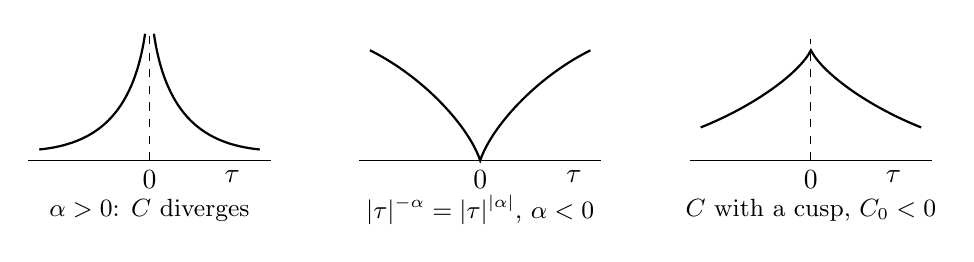
\begin{tikzpicture}[scale=0.7]
  \draw (-2.2,0) -- (2.2,0); \draw[dashed] (0,0) -- (0,2.4);
  \draw[thick] (-0.08,2.3) .. controls (-0.3,0.8) and (-1,0.3) .. (-2,0.2);
  \draw[thick] (0.08,2.3) .. controls (0.3,0.8) and (1,0.3) .. (2,0.2);
  \node[below] at (0,0) {$0$}; \node[below] at (1.5,0) {$\tau$};
  \node[font=\small] at (0,-0.9) {$\alpha>0$: $C$ diverges};
  \begin{scope}[xshift=6cm]
  \draw (-2.2,0) -- (2.2,0);
  \draw[thick] (-2,2) .. controls (-1,1.5) and (-0.2,0.6) .. (0,0) .. controls (0.2,0.6) and (1,1.5) .. (2,2);
  \node[below] at (0,0) {$0$}; \node[below] at (1.7,0) {$\tau$};
  \node[font=\small] at (0,-0.9) {$|\tau|^{-\alpha} = |\tau|^{|\alpha|}$, $\alpha<0$};
  \end{scope}
  \begin{scope}[xshift=12cm]
  \draw (-2.2,0) -- (2.2,0); \draw[dashed] (0,0) -- (0,2.2);
  \draw[thick] (-2,0.6) .. controls (-1,1.0) and (-0.2,1.6) .. (0,2) .. controls (0.2,1.6) and (1,1.0) .. (2,0.6);
  \node[below] at (0,0) {$0$}; \node[below] at (1.5,0) {$\tau$};
  \node[font=\small] at (0,-0.9) {$C$ with a cusp, $C_0<0$};
  \end{scope}
\end{tikzpicture}
\diagramcaption{Specific heat near $T_c$ for $\alpha>0$ and for $\alpha<0$.}
\end{diagram}

$\beta<1$ for all of the models and systems studied, which is reflected in the curves for the order
parameter, e.g.\ the magnetization $M(T)$, in these phase transitions. The smaller the exponent $\beta$
is, the more rapid the onset of magnetic order as $T$ decreases below $T_c$, e.g.\ 2D Ising ($q = 2$
Potts): $\beta = \frac18$; 2D $q = 3$ Potts: $\beta = \frac19$; 2D $q = 4$ Potts: $\beta = \frac1{12}$; 3D
Ising: $\beta\simeq 0.325$; 3D $O(3)$: $\beta\simeq 0.37$.

\subsection{The renormalization ``group'' is a semigroup}

The Kadanoff block-spin construction is the basis of the real-space renormalization group (RG).
However, the term ``group'' is a misnomer here. Recall the definition of a group $G$:

\paragraph{Definition.} A group $G$ is a set of elements $g,h,\ldots$ with an operation such that
\begin{enumerate}[label=(\arabic*)]
  \item $g\cdot h\in G$ (closure property);
  \item $\exists\,1$ such that $g\cdot 1 = 1\cdot g = g$ (existence of identity);
  \item for each $g\in G$, $\exists\,g^{-1}$ such that $g\cdot g^{-1} = g^{-1}\cdot g = 1$ (existence of
    inverse);
  \item if $g,h,k\in G$, then $g\cdot(h\cdot k) = (g\cdot h)\cdot k$ (associativity).
\end{enumerate}
We can regard the block-spin operation $R_b$ with blocking parameter $b = L$ as the basic element, and
this satisfies closure: $R_b(R_b) = R_b^2 = R_{b^2}$. If one only includes $R_b$ actions, then there is
neither an identity nor an inverse, so the RG is a semigroup. If one extends the definition to include
not applying $R_b$, then there is an identity, so then the RG is a semigroup with identity, i.e.\ a
monoid.

To see why there is no inverse, let us recall the basic operation of $R_b$: the prescription replaces a
set of spins on the original lattice by a single spin on the blocked lattice. For example, with an Ising
model, the spin after the blocking step is again an Ising spin, $\pm1$, determined by a majority rule:
\begin{equation*}
  \begin{array}{cc}+&+\\+&+\end{array}\to +,\quad
  \begin{array}{cc}+&+\\+&-\end{array}\to +,\quad
  \begin{array}{cc}+&-\\+&+\end{array}\to +,\quad
  \begin{array}{cc}-&+\\+&+\end{array}\to +,\quad
  \begin{array}{cc}+&+\\-&+\end{array}\to +.
\end{equation*}
All 5 of these Ising spin configurations on the original lattice $\Lambda$ give the same Ising spin on the
blocked lattice, and similarly with the opposite-sign spins. Hence, knowing the value of the Ising spin
$\pm$ on the blocked lattice, we cannot go backward to determine the spin configuration on the original
lattice. (In actual implementations of the real-space RG on the square or cubic lattice, one typically
uses a random number ``tie-breaker'' to deal with ties such as
$\begin{smallmatrix}+&+\\-&-\end{smallmatrix}$, $\begin{smallmatrix}-&-\\+&+\end{smallmatrix}$,
$\begin{smallmatrix}+&-\\-&+\end{smallmatrix}$, $\begin{smallmatrix}-&+\\+&-\end{smallmatrix}$.)
This is not a serious problem if the blocking takes place in the deep interior of a correlated region of
spins, since they are almost all $+$ or all $-$, but it is significant at border regions between $+$ and
$-$ regions. Note that on a triangular lattice one does not need a tie-breaker, since the net spin will
be $+$ or $-$: the triangles $(+,+,+)$, $(+,+,-)$, $(+,-,+)$, $(-,+,+)$ all map to $+$. But the same
comment about the non-existence of an inverse applies.

A corresponding statement holds for the blocking transformation applied to a continuous spin system: e.g.\
the pairs of $O(N)$ spins $(\nwarrow\nearrow)$ and $(\nearrow\nwarrow)$ on the initial lattice are both
mapped to the same spin $\uparrow$ on the blocked lattice. So the real-space renormalization group is
really a semigroup, with no inverse defined.
